\section{DisplayCAL}
DisplayCAL\footnote{\href{https://displaycal.net/}{https://displaycal.net/}} è un software libero di calibrazione e profilazione di display basato su ArgyllCMS\footnote{\href{https://www.argyllcms.com/}{https://www.argyllcms.com/}}.

Lo scopo principale di questa applicazione è quella di misurare l'accuratezza dei colori del display utilizzando un colorimetro o uno spettrofotometro tra quelli supportati da ArgyllCMS e generare un profilo di colore ICC che può essere utilizzato nel sistema operativo per fornire dei colori più accurati. Oltre alla calibrazione, può generare anche dei report che mostrano il gamut del display, le curve di gamma, e molto altro, secondo molti standard.

La figura \ref{fig:displaycal_report_example} mostra un esempio di report generato da DisplayCAL riguardante l'accuratezza dei colori. Il test consiste nel visualizzare una serie di colori e calcolare la differenza tra il colore visualizzato e quello inteso utilizzando qualche tecnica come Delta-E 1976, tenendo conto dello spazio colore in cui deve essere visualizzato.

\begin{figure}[h]
	\centering
	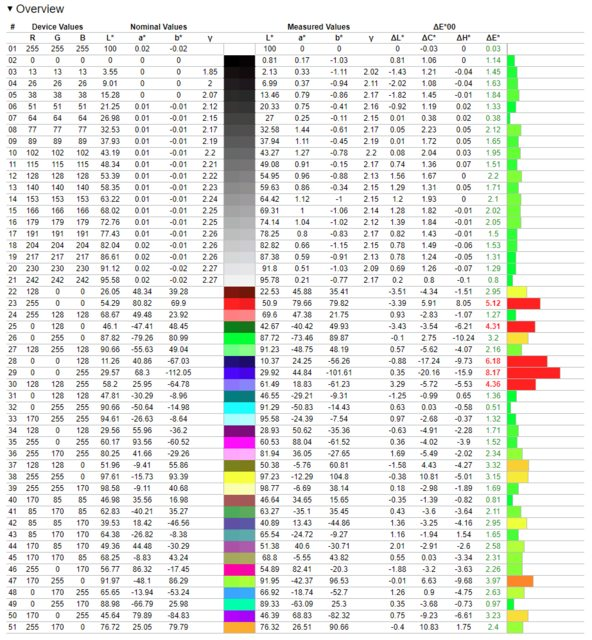
\includegraphics[width=\textwidth]{Chapter02/res/displaycal_report_example.jpg}
	\caption{Esempio di report sull'accuratezza dei colori}
	\label{fig:displaycal_report_example}
\end{figure}

Siccome questo software si concentra sulla qualità dell'immagine e soprattutto dei colori, il suo obiettivo è diverso rispetto a quello di Nvidia LDAT e di OpenLDAT, e non implementa alcun test riguardante le tempistiche del display e del sistema (Marzo 2021). I dispositivi supportati da DisplayCAL inoltre sono molto più sofisticati e piuttosto costosi, con i modelli più economici (dei colorimetri a tre canali) che partono da circa 100€.
